%%%%%%%%%%%%%%%%%%%%%%%%%%%%%%%%%%%%%%%%%
% Memo
% LaTeX Template
% Version 1.0 (30/12/13)
%
% This template has been downloaded from:
% http://www.LaTeXTemplates.com
%
% Original author:
% Rob Oakes (http://www.oak-tree.us) with modifications by:
% Vel (vel@latextemplates.com)
%
% License:
% CC BY-NC-SA 3.0 (http://creativecommons.org/licenses/by-nc-sa/3.0/)
%
%%%%%%%%%%%%%%%%%%%%%%%%%%%%%%%%%%%%%%%%%

\documentclass[letterpaper,11pt]{texMemo} % Set the paper size (letterpaper, a4paper, etc) and font size (10pt, 11pt or 12pt)

\usepackage{parskip} % Adds spacing between paragraphs
\usepackage[colorlinks]{hyperref}
\usepackage{graphicx}
\usepackage{float}
\usepackage{listings}
\hypersetup{citecolor=DeepPink4}
\hypersetup{linkcolor=red}
\hypersetup{urlcolor=blue}
\usepackage{cleveref}
\setlength{\parindent}{15pt} % Indent paragraphs

%----------------------------------------------------------------------------------------
%	MEMO INFORMATION
%----------------------------------------------------------------------------------------

\memoto{Dr.Randy Hoover} % Recipient(s)

\memofrom{Benjamin Lebrun, Benjamin Garcia} % Sender(s)

\memosubject{Lab Assignment 4: Remote Control} % Memo subject

\memodate{\today} % Date, set to \today for automatically printing todays date

%\logo{\includegraphics[width=0.1\textwidth]{logo.png}} % Institution logo at the top right of the memo, comment out this line for no logo

%----------------------------------------------------------------------------------------

\begin{document}

\maketitle % Print the memo header information

%----------------------------------------------------------------------------------------
%	MEMO CONTENT
%----------------------------------------------------------------------------------------

\section*{Introduction}
%This section \textit{briefly} communicates what you have been asked to accomplish in the lab, how you approached it, and what results you saw. This is \textbf{not} an area for manifestos.

This project required us to create a console application that would read whether a pin was connected to a 5-volt source (would read 'high') or was not (would read 'low'). The application was also required to allow setting other pins to output high/low and to drive LEDs. The console portion was required to output an appropriate error message if invalid inputs were provided. The types of invalid inputs that could be detected included invalid commands (those other than 'set' or 'read'), invalid pins (set operations were only valid for pins 8 and 10, while read operations were only valid for pins 9 and 11), and invalid states (anything other than 'high' or 'low').

We began by creating an input interrupt handler, a buffer for input, and a stream object for output. This allowed us to read input from the interrupt handler into the buffer, and to output information back to the console using the stream object. Once basic IO was handled, we wrote code to tokenize the input on spaces and check the inputs for validity. If input was valid, the appropriate state values were set and execution continued. If input was invalid, the state flags would be set to error values and an appropriate message would be output. Once input processing was finished, low-level IO functions would be invoked based on the command and pin specified, and read or write operations with the pins were performed. After all processing and reading/writing, a message indicating the result of the command is printed to the terminal, and the program awaits further input.

Physically, we use push-buttons connected to the breadboard to handle reading high or low values from pins 9 and 11. If the button is pressed, the pins read 'high' as they are connected to the 5-volt source on the board, otherwise they read low. We have attached LEDs to the buttons to provide a visible indication of when the pins should read 'high' or 'low'.

On reset, the output pins start low, and the input pins are pulled low by the internal pull-down resistors. This means that the LEDs begin off and the read pins are 'low' before any user input is performed. When pin 8 is set high by the 'set 8 high' command, our blue LED will turn on. Similarly, when pin 10 is set high, the red LED will turn on. If either is set low by the 'set (8|10) low' command, the respective LED will turn off. The read pins (9 and 11) read low until their respective buttons are pushed. When the button for pin 9 is pressed, the yellow LED will turn on, and a read from the pin will report 'high'. Similarly, when the button for pin 11 is pressed, the green LED will turn on, and a read on pin 11 will report 'high'.


\section*{Equipment}
This lab required the following equipment:
\begin{itemize}
\item 4 resistors (220$\Omega$)
\item 4 LEDs
\item 2 push-buttons
\item 8 wires (male-male)
\item 1 USB-A to USB-B cable
\item 1 breadboard
\item 1 Arduino UNO (ATMega328P)
\item AVR 8-bit GCC toolchain
\item Putty
\end{itemize}

\subsection*{Configuration}
For the circuit configuration we have a simple line from pins 8 and 10 from the Arduino unit to the LEDs behind two
resistors to ground. For our voltage inputs we have a simple normally open push button switch. For each input, we have
a 5 volt rail entering into one side of the push button, the other side has a hardware indication LED connected to
ground with a pulldown resistor and our line to input on the arduino. When the button is pressed, it should put 5
volts of potential on the rail and appropriately light the LED.

\begin{figure}[!ht]
\begin{center}
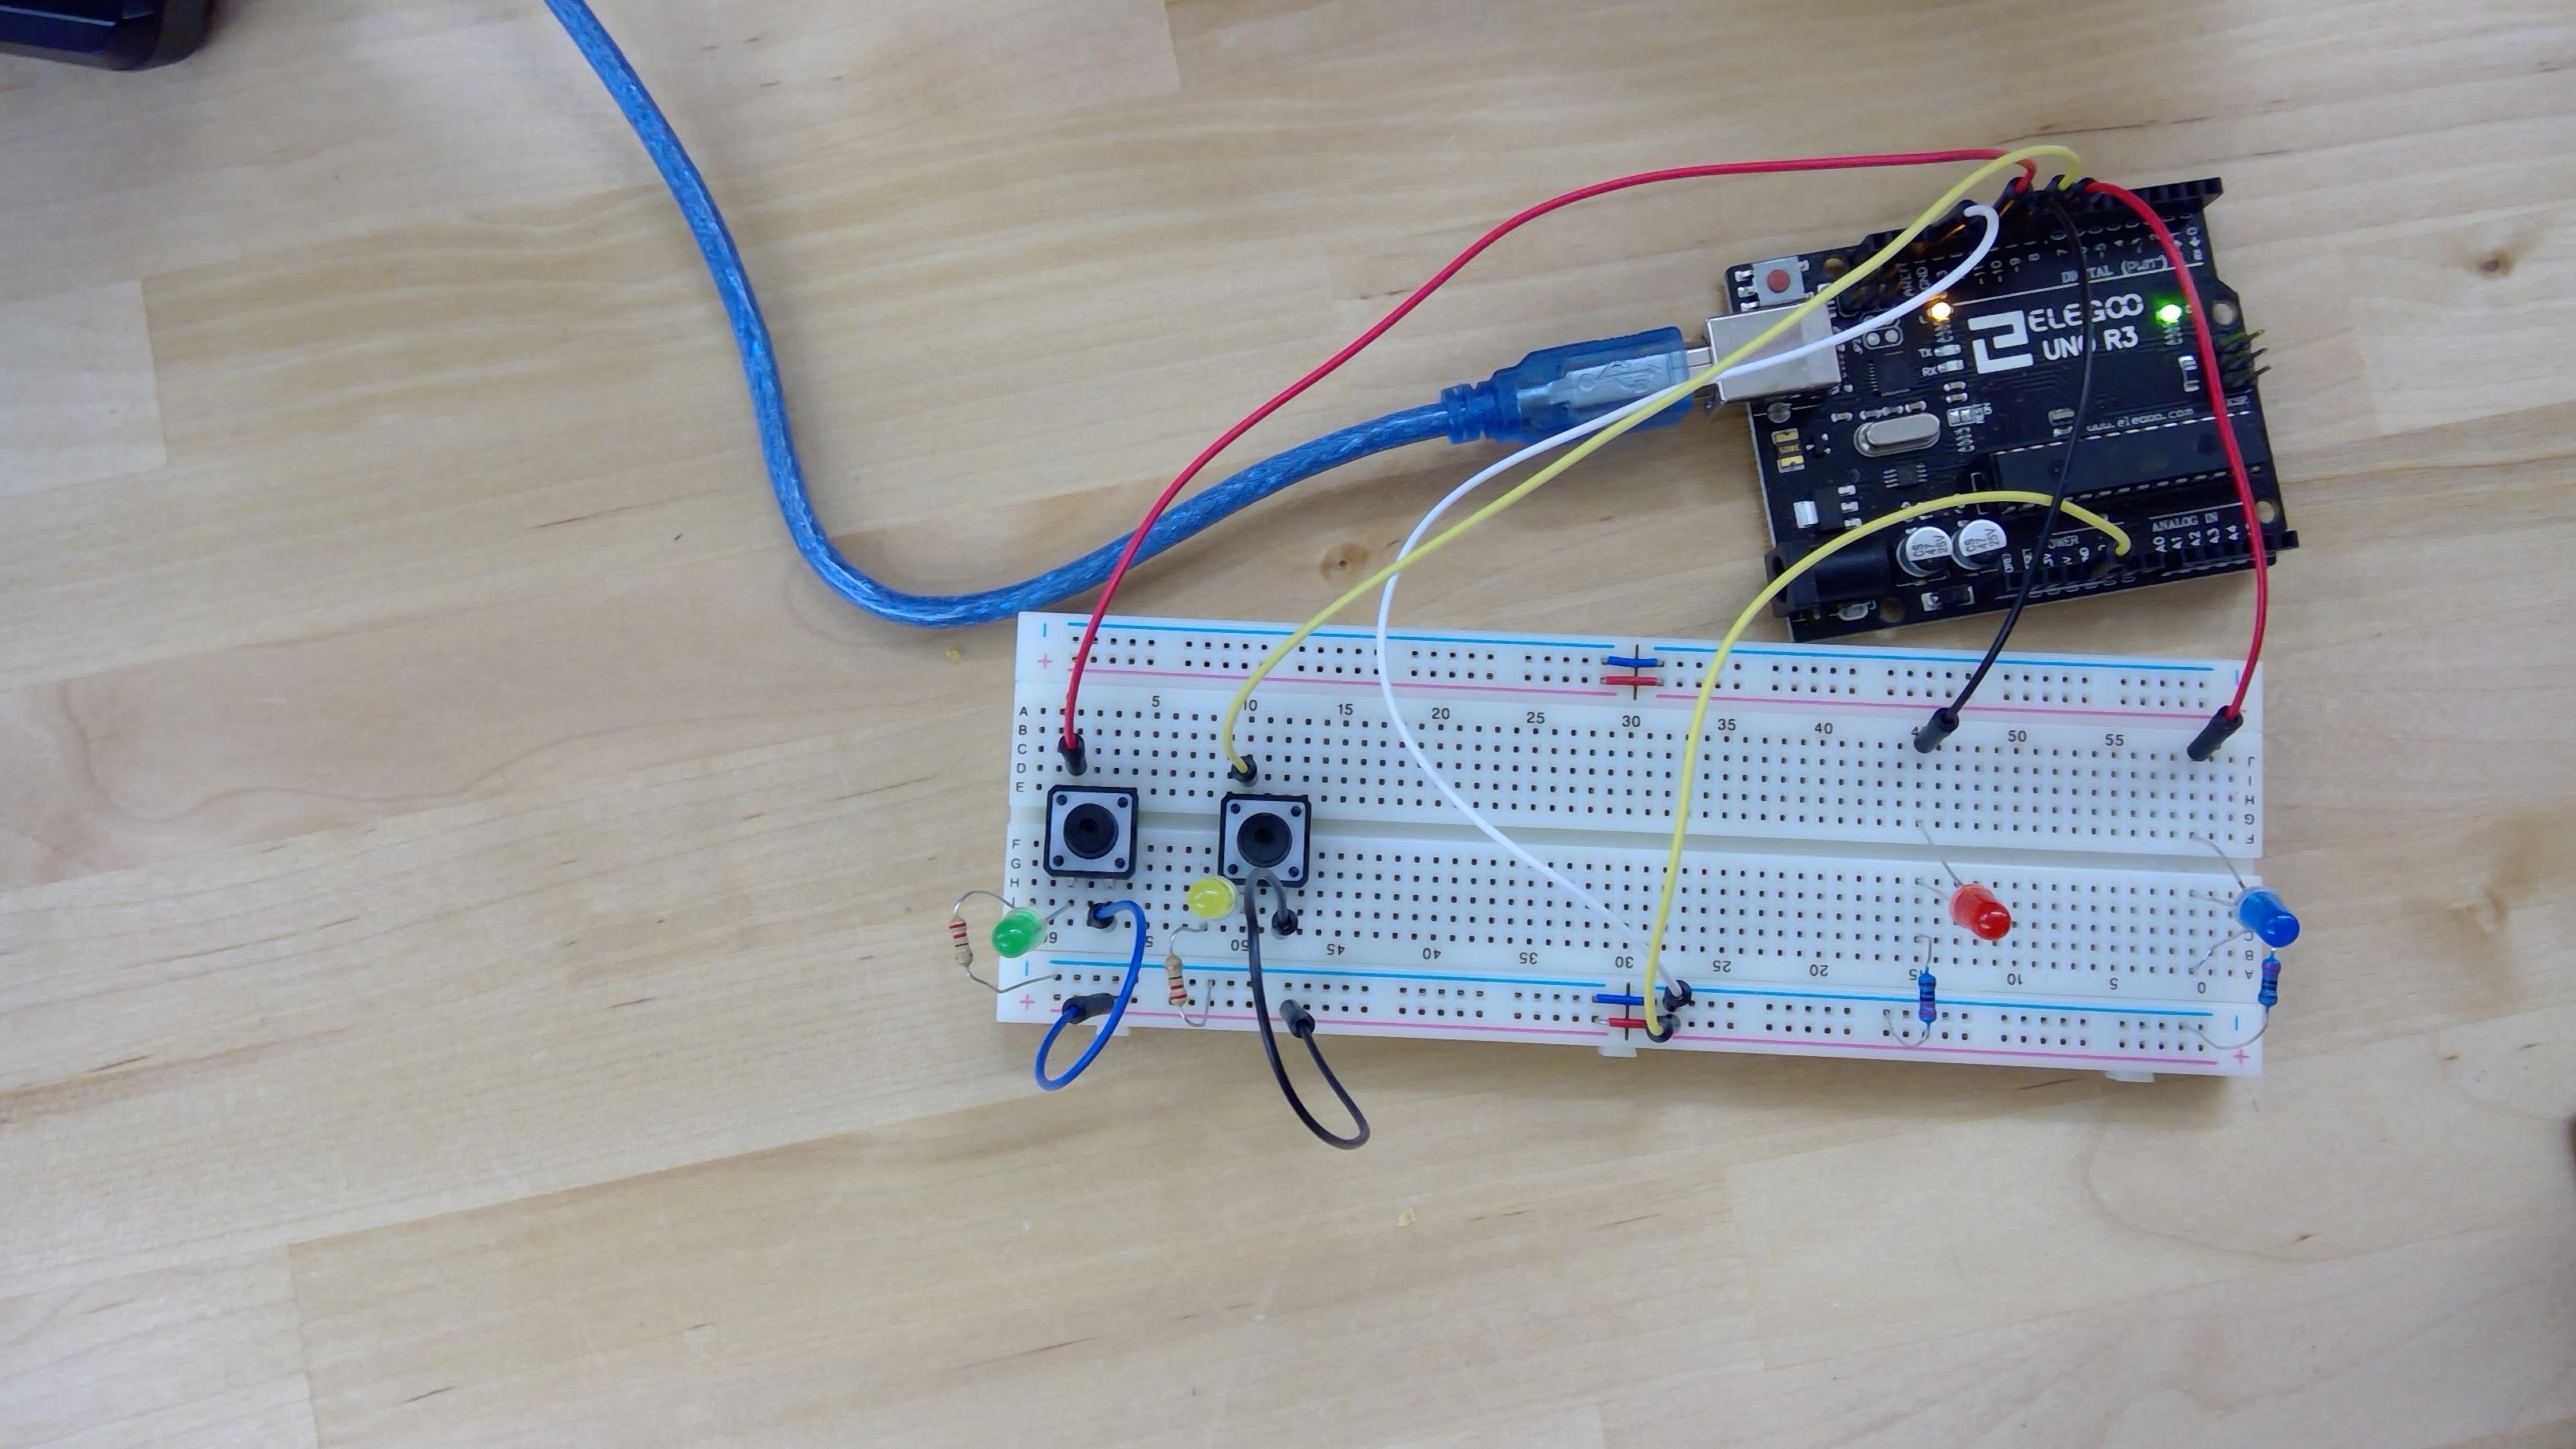
\includegraphics[width=\linewidth]{./configuration.jpg}
\caption{Picture of the wiring setup}
\end{center}
\end{figure}

\newpage
\section*{Implementation}

\subsection*{int main(void)}
Performs startup logic by calling \textit{initUART} and \textit{initPins}, then loops forever using a 'while(1)' empty loop. After startup, program is entirely interrupt driven. 

\subsection*{ISR(USART\_RX\_vect) (interrupt)}
Every character of user input is handled by this function, which inserts the character into the \textit{iobuff} character array. The program expects input to be terminated with a carriage-return ('\verb+\r+'), at which point the \textit{processMessage} will handle the input, and the buffer will be cleared.
\subsection*{processMessage(char* str)}
This function tokenizes the input and calls a series of state modifying functions that will each perform error checking. If the input passes validation checks, the command is executed, and the appropriate operations are performed.
Invokes \textit{setMessageType}, \textit{setPinNumber}, and \textit{setPinMode} to perform error checking and state setting. If input is empty the invalid command message is printed. The standard library \textit{strtok} function is used to parse the input, and three pointers \textit{combuff}, \textit{pinbuff}, and \textit{setbuff} are used to access the relevant segments.
\subsection*{void setMessageType(char* str)}
Checks the command segment of the input to determine if it is one of the valid commands. If it is not, the \textit{type} state variable is set to MSG\_INV and the \textit{inv} state variable is set to INVALID\_COMMAND. Otherwise the \textit{type} variable is set to MSG\_SET or MSG\_READ if the command was 'write' or 'read' respectively. Input can be capitalized (HIGH) or lowercase (low) but not mixed (HiGh).
\subsection*{void setPinNumber(char* str, enum MSG\_TYPE mode)}
Once the command has been validated, the next segment of the input is processed to determine which pin the operation applies to (assuming the pin is permissible for that operation). If the pin is invalid for the command, the \textit{type} variable is set to MSG\_INV, the \textit{inv} variable is set to INVALID\_PIN, and \textit{pin} is set to PIN\_NONE. Otherwise pin will have one of the following values:
\begin{itemize}
\item PIN\_EIGHT\\
\item PIN\_NINE\\
\item PIN\_TEN\\
\item PIN\_ELEVEN
\end{itemize}
\subsection*{setPinMode(char* str)}
If the selected command was 'write' then this function determines if the pin is to be set 'high' or 'low'. if the input is neither 'high' nor 'low' the \textit{pin} value is set to NONE, the \textit{type} variable is set to MSG\_INV, and \textit{inv} is set to INVALID\_STATE.
\subsection*{void initUART()}
Configure the UART baud rate and RX Complete interrupt. 
\subsection*{void printMsg()}
Prints a message to the terminal using the \textit{mystdout} stream based on the state variables. Format strings are stored in strings.h and accessed using the state variables to index into arrays of pointers to the strings. Strings are combined using \textit{fprintf}.
\subsection*{static int uart\_putchar(char c, FILE* stream)}
Stream input function for \textit{mystdout}. Sends parameter characters one by one through the UART to the terminal.
\subsection*{enum MSG\_TYPE}
Enumeration of message types. Used to determine what message to print on output and what operation is being performed. Values are used to access the \textit{uiMsgs} array to retrieve format strings for use in \textit{printMsg};
\subsection*{enum TGT\_PIN}
Enumeration of pins usable by the program. Operations on pins use these values to indicate which pin is the target of a read or write operation. Usable as an index into the \textit{pinMsgs} array of strings representing the pin name.
\subsection*{enum SET\_TYPE}
Enumeration of values a pin can have. Can be used as an index into the \textit{stateMsgs} array of strings containing state messages. The NONE value is used in error cases, while HIGH and LOW correspond to their respective pin states.
\subsection*{enum INVALID\_TYPE}
Used with the MSG\_INV value of the MSG\_TYPE enum to specify why an input was invalid. Indexes into the \textit{errorMsgs} array to specify which string to use in the MSG\_INV format string.
\subsection*{void initPins()}
Initializes the states of the pins used in the program. All pins are written low to begin, and (labeled) pins 8 and 10 are marked for output.
\subsection*{int ReadPinDigital(enum TGT\_PIN pin}
Handles reading from the pin indicated by \textit{pin} and returns 0 if the pin is low or 1 if the pin is high. If the pin is invalid for the read operation -1 is returned.
\subsection*{int WritePinDigital(enum TGT\_PIN pin, enum SET\_TYPE mode}
Handles writing to the pin indicated by \textit{pin}. Sets the pin to the mode indicated by \textit{mode} and returns 1 if the pin is valid, otherwise returns 0 indicating an invalid setup.
\subsection*{strings.h}
We use strings.h to hold several c-strings for handling output to the terminal. We access these strings by means of arrays of pointers to the strings, where the arrays can be accessed by enum values. This makes the code more general and easier to work with.

\section*{Discussion}

    The first of many troubles, for user input we had an issue with carriage returns versus newlines, 
how our code would determine the end of a buffer input. We initially checked only for \verb+'\n'+ inside of our
buffer and initiated a buffer flush and process the string. The buffer was failing to flush and read properly,
when we checked for a carriage return instead of a newline character our buffer was properly able to flag the 
end of a user command and begin processing the string
    
    Pin set configuration and port directions and masks were the next issue. This was simply a lapse in judgement
on the programmer's part in how to properly twiddle bits around in code to single out the necessary register bit.

    Pulldown/Pullup internal resistor with our input ports was another fabulous discovery. We used buttons to 
activate our pins however we discovered that their results weren't entirely deterministic. To solve this and add
a nice feature on top we used an external puldown resistor paired with an LED to indicate when power was flowing
through the switch as a hardware fallback indicator.

    In the real world, many components use UART communication where more advanced or complicated data must be 
comunicated. This also applies to communication between computers or other microcontrollers on a unified system.
Because of this, we must know how to also communicate using different interfaces, such as GPIO when UART is either
occupied or unavailable. 

    In pursuit of this, we learned how to utilize processing commands with UART communication between two 
machines in this lab. We also explored reading information from external sources by using the GPIO pins 
on our microcontroller board.


\newpage
\section*{Responses}
\begin{enumerate}
    \item Checksums are often used to verify the integrity of transmitted data. What is a check-
sum? Walk through the calculation of the modular sum checksum for the ASCII string
”CENG447”. Now generate a longitudinal parity byte for the same string.
 
    A checksum is a piece of data used to test incoming data for transmission 
integrity. There's several ways to calculate a checksum, one example of a checksum is a 
modular sum checksum. This simple checksum adds the digits of the message together, continuously
performing modulus with every sum until we have a final remainder.

    For our test string "CENG447", using a modular sum checksum, induvidually
adding together each letter and modulating the result continuously by 255, our checksum comes out
to 189.

    \item Several different communication standards are used for inter-system serial communication,
most notably RS-232 and RS-485. What are the differences between RS-232, RS-485, and the
UART on our ATMega328Ps?

    For the serial standards RS-232 and RS-485, the major difference between these two standards is
the voltage level of the devices that use these standards. The RS-485, uses an activation voltage of
200 mV in either the positive and negative direction, but the RS-232 uses a positive/negative voltage
of 5V, both activate as digital 1 on the negative edge.

    The RS-232 has a lower minimum impedance, but has a smaller transmission range across it's cable
and a smaller transmission rate. The RS-485 has a superior transmission cable length and superior
transmission rate.

    \item Our ATMega328Ps have built-in pullup resistors. What is a pullup/pulldown resistor, and
what is a risk of not using them? How does one enable the ATMega328P’s internal pullup
resistors?

    A pullup or pulldown resistor assist the signal in being able to hold either a grounded or
reference voltage signal. Without an internal or external pullup or pulldown resistor, the pin
generally "floats" or does not hold either signal discriminately, and could return improper
digital readings when accessed. To enable the board's internal pullup resistor, while the pin
is in read mode, we write a 1 to the necessary pin bit with its appropriate \textit{PORTX} 
register, replacing \textit{X} with our port.

\end{enumerate}

\section*{Appendices}
The following files are included as appendices:
\begin{itemize}
\item main.c - entry file, manages initialization logic and interrupt handling
\item pinops.h - header file for the pin operations file 
\item pinops.c - handles pin operations
\item strings.h - has static string constants for testing and printing
\item msg_types.h - has enumerations for program state and output
\end{itemize}
\newpage

\section*{Appendix A: main.c}
\begin{tiny}
\lstinputlisting{../main.c}
\end{tiny}
\newpage
\section*{Appendix B: pinops.h}
\begin{tiny}
\lstinputlisting{../pinops.h}
\end{tiny}
\newpage
\section*{Appendix C: pinops.c}
\begin{tiny}
\lstinputlisting{../pinops.c}
\end{tiny}
\newpage
\section*{Appendix D: msg_types.h}
\begin{tiny}
\lstinputlisting{../msg_types.h}
\end{tiny}
\newpage
\section*{Appendix D: strings.h}
\begin{tiny}
\lstinputlisting{../strings.h}
\end{tiny}
\end{document}
